\section{The Canonical Decomposition-Recombination Plan}
\label{sec:DRP}

\newcommand{\usestwod}{\todo{Uses 2D requirement:}}
\renewcommand{\usestwod}{}

\subsection{Theory}

In the problem of the optimal DR-Plan there is generally not a unique plan.
% Indeed, we will prove a union of $N$ well-constrained subgraphs will result in $N$ unique plans, but that at the $N^{\text{th}}$ level of the tree it will always be the same. Therefore, all choices of decomposition are in some sense equivalent. The theorem we seek to prove is thus:
However, we will show that regardless of which children are chosen for the plan, so long as they satisfy the definition of an optimal DR-plan, the recombination will require solving of the same systems. Being the smallest such structure that offers this, the definition of an optimal DR-plan could be considered the canonical DR-plan.
% To assist in showing this, we prove this core theorem throughout this section:

In this section, we discuss 2D bar-joint graphs. All vertex weights are $2$, all edge weights are $1$, and constant $k= -{{3}\choose{2}}=-3$. Trivial graphs are a single vertex and empty set. Furthermore, 2D well-constrained graphs must be connected.
% The greatest density of a 2D well-constrained graph is $-2$ (the vertex). The other disconnected part of the graph would need to have a density of $-1$, which is over-constrained and not possible in a well-constrained graph (because there is no trivial graph with that density).



\begin{theorem}\label{theorem:main}
Given a well-constrained 2-dimensional bar-joint graph $G$, for node $C$ in $OptimalDRP(G)$ and the children of $C$ in $CompleteDRP(C)$ labeled as $C_1,\ldots,C_N$
\begin{enumerate}
    \item if $C_i \cap C_j$ is trivial then all $C_1,\ldots,C_N$ are children of $C$ in $OptimalDRP(G)$
    \item if $C_i \cap C_j$ is well-constrained then any two out of $C_1,\ldots,C_N$ will be the only children of $C$ in $OptimalDRP(G)$.
\end{enumerate}
This covers all potential cases.
\end{theorem}

\begin{proof}
Remark \ref{lemma:union_intersection} shows that the intersection of any two well-constrained subgraphs (such as $C_i$ and $C_j$) can only result in trivial or well-constrained subgraphs. Therefore, these are the only possibilities to consider.


\begin{enumerate}
\item
% In a valid DR-plan, all children must be proper subgraphs. Therefore, for the union to be the parent (and satisfy the conditions of a DR-plan) there must be at least two children.
It follows directly from Lemma \ref{lemma:wc_intersection_makes_all_wc} that if there exists $C_i, C_j$ such that $C_i \cup C_j$ is well-constrained, then the smallest fan-in at this node can be made by selecting any two $C_i, C_j$.
% you found a tree with only 2 children.
% Clearly, this is the optimal choice at this level.
However, for it to be a solution to $OptimalDRP(G)$, it must not affect the maximum fan-in for any descendant.

Take $D=\bigcap_{k\in N}{C_k}$ and $R_k=C\setminus C_k$. Suppose we select $i$ and $j$, where $i\neq j$, as the children. Since
% \[C_i=Idc\left(C,D\cup\bigcup_{k\in N\setminus\{i\}}{R_k}\right)\]
% the children of this node will be
% \[Idc\left(C,D\cup\bigcup_{k\in N\setminus\{i,m\}}{R_k}\right)\]
% and
% \[Idc\left(C,D\cup\bigcup_{k\in N\setminus\{i,n\}}{R_k}\right)\]
$C_i=Idc\left(C,D\cup\bigcup_{k\in N\setminus\{i\}}{R_k}\right)$
the children of this node will be
$Idc\left(C,D\cup\bigcup_{k\in N\setminus\{i,m\}}{R_k}\right)$
and
$Idc\left(C,D\cup\bigcup_{k\in N\setminus\{i,n\}}{R_k}\right)$
for arbitrary $m$ and $n$, where $m\neq n$. This continues for $N-1$ levels total, always with fan-in of two (the minimum possible), at which point every descendant of $C$ is some $Idc(C,D\cup R_k)$.

%%%%%%%%%%%%%%%

\item
Take $X\subset \{1,\ldots,N\}$ and $D=\bigcup_{i\in X}{C_i}$. If $D\neq C$ but it was well-constrained, then we just found a larger proper subgraph and the graphs in the set were not vertex-maximal to begin with.

\usestwod
By Lemma \ref{lemma:uc_intersection_makes_all_uc}, if $C_i \cap C_j$ is trivial then for $k\notin X$, $D\cap C_k$ must be one or more trivial subgraphs. Since $C_k=C\cap C_k=D\cap C_k$, by definition of a DR-plan, the assumption that $C_k$ is well-constrained has been contradicted. Thus, $X$ must be all of $\{1,\ldots,N\}$.
\end{enumerate}
\end{proof}

The following subsections provide the supporting proofs.



%%%%%%%%%%%%%%%%%%%%%%%%%%%%%%%%%%%%%%%%%%%%%%%%%%%%%%%%%%%%%%%%
%%%%%%%%%%%%%%%%%%%%%%%%%%%%%%%%%%%%%%%%%%%%%%%%%%%%%%%%%%%%%%%%
%%%%%%%%%%%%%%%%%%%%%%%%%%%%%%%%%%%%%%%%%%%%%%%%%%%%%%%%%%%%%%%%

\subsubsection{Relationships for the Union and Intersection of Well-Constrained Subgraphs}
\label{sec:union_intersection}

% This is general, not for 2d
\begin{remark}\label{lemma:union_intersection}
If $F_i$ and $F_j$ are well-constrained subgraphs of the same well-constrained graph $F$, then it must be that:
\begin{enumerate}
    \item $F_i\cup F_j$ is not trivial.
    \item $F_i\cup F_j$ is under-constrained if and only if $F_i\cap F_j$ is trivial.
    \item $F_i\cup F_j$ is well-constrained if and only if $F_i\cap F_j$ is well-constrained.
    \item $F_i\cap F_j$ is not under-constrained.
\end{enumerate}
\end{remark}

\begin{proof}
Note that, by definition, $d(F_i)=k$ and $d(F_j)=k$. Also, $d(F_i\cap F_j)=d(F_i)+d(F_j)-d(F_i\cup F_j)$.
\begin{enumerate}
    \item By definition of trivial graph; if $F_i\cup F_j$ were trivial, then $F_i$ and $F_j$ must be trivial.

    \item \textit{Forward direction:} Since $F_i\cup F_j$ is under-constrained and a subgraph of well-constrained $F$, it must be that $d(F_i\cup F_j)=l<k$. Therefore $d(F_i\cap F_j)=2k-l>k$. This means $F_i\cap F_j$ is trivial. \textit{Reverse direction:} We know that $d(F_i\cap F_j)>k$ because it is trivial. By the same math, we find that $d(F_i\cup F_j)<k$, showing it is under-constrained.

    \item \textit{Forward direction:} We have that $d(F_i\cup F_j)=k$, therefore $d(F_i\cap F_j)=k$. Being a subgraph of well-constrained $F$, $F_i\cap F_j$ is also well-constrained. \textit{Reverse direction:} By the same math, we find that $d(F_i\cup F_j)=k$ and, since it is also a subgraph of $F$, it is well-constrained.

    \item Subgraphs of well-constrained graph $F$ can only be trivial, under-constrained, or well-constrained. So it follows from the above that an under-constrained intersection is not possible.
\end{enumerate}
\end{proof}





%%%%%%%%%%%%%%%%%%%%%%%%%%%%%%%%%%%%%%%%%%%%%%%%%%%%%%%%%%%%%%%%
%%%%%%%%%%%%%%%%%%%%%%%%%%%%%%%%%%%%%%%%%%%%%%%%%%%%%%%%%%%%%%%%
%%%%%%%%%%%%%%%%%%%%%%%%%%%%%%%%%%%%%%%%%%%%%%%%%%%%%%%%%%%%%%%%

\subsubsection{Inferring Parent Structure from Union and Intersection of Children}
\label{sec:infer_parent}


\begin{lemma}\label{lemma:wc_intersection_is_C}
$C_i\cup C_j$ is well-constrained if and only if $C_i\cup C_j = C$.
\end{lemma}

\begin{proof}
%I wouldn't do the forward and backward direction italics, or say proof by contradiction. Just start the first paragraph with Suppose C_i union C_j is well constained maximal proper and assume it is not C. 
\textit{Forward direction:} Proof by contradiction. If the $C_i\cup C_j$ was well-constrained but $C_i\cup C_j \neq C$, we would have found a larger well-constrained proper subgraph containing them; namely, $C_i\cup C_j$ or something containing it. The two original subgraphs could not have been vertex-maximal proper.

\textit{Reverse direction:} $C$ is either some non-leaf node (well-constrained by definition of a DR-plan) or $G$ itself (well-constrained by definition of the problem). Thus, $C_i\cup C_j$ is well-constrained.
\end{proof}

\begin{corollary}\label{corollary:no_edges_between_diff}
Let us say $R_i=C\setminus C_i$ and $R_j=C\setminus C_j$. If $C_i\cup C_j$ is well-constrained, then there can be no edges in $C$ between the vertices of $R_i$ and $R_j$.
\end{corollary}

\begin{proof}
Lemma \ref{lemma:wc_intersection_is_C} shows that $C_i\cup C_j$ must equal the entire parent $C$.
\end{proof}



\begin{lemma}\label{lemma:wc_intersection_makes_all_wc}
If $C_i\cup C_j$ is well-constrained, then $\forall k: C_i\cup C_k$ is well-constrained.
Alternatively, if $C_i\cup C_j=C$, then $\forall k: C_i\cup C_k=C$.
\end{lemma}

\begin{proof}
In appendix (\ref{sec:appendix}).
\end{proof}



\begin{lemma}\label{lemma:uc_intersection_makes_all_uc}
If $C_i\cap C_j$ is trivial, then $\forall k: C_i\cap C_k$ is trivial.
\end{lemma}

\begin{proof}
By Lemma \ref{lemma:union_intersection}, if some $C_i\cap C_k$ is not trivial, then it must be well-constrained. Then, by Lemma \ref{lemma:wc_intersection_makes_all_wc}, all of the intersections are well-constrained. This contradicts the statement that $C_i\cap C_j$ is trivial.
\end{proof}


%%%%%%%%%%%%%%%%%%%%%%%%%%%%%%%%%%%%%%%%%%%%%%%%%%%%%%%%%%%%%%%%
%%%%%%%%%%%%%%%%%%%%%%%%%%%%%%%%%%%%%%%%%%%%%%%%%%%%%%%%%%%%%%%%
%%%%%%%%%%%%%%%%%%%%%%%%%%%%%%%%%%%%%%%%%%%%%%%%%%%%%%%%%%%%%%%%

% \subsubsection{Further Results}


% \begin{corollary}
% Take $\bigcap_{k=1}^N{C_k}$ to be the graph $D$. If $D$ is well-constrained, then $D$ will be a descendant of every $C_k$.
% \end{corollary}

% \begin{proof}
% Explained in Theorem \ref{theorem:main_wellconstrained}.
% \end{proof}


% \begin{corollary}
% $\forall i,j\in [1,\ldots,N]$ if $i\neq j$ there are no edges in $C$ between the vertices in subgraphs $C\setminus C_i$ and $C\setminus C_j$.
% \end{corollary}

% \begin{proof}
% Further constraints between them would imply $C_i \cup C_j$ is a subgraph of $C$, but lemma \ref{lemma:wc_intersection_is_C} proves is the entire graph.
% \end{proof}

% \begin{proof}
% It follows from Theorem \ref{theorem:main_trivial} that if the intersection of any two well-constrained vertex-maximal proper subgraphs of $C$ are well-constrained then all of them are well-constrained or $\emptyset$.
% \end{proof}

% Figure idea: Large node in the middle with weight $k$. Several other graphs with weight $a, b, c, d\ldots$ attached radially by single edges with weights $a, b, c, d\ldots$ respectively. Circle each vertex-maximal subset.

% $\forall k\in [1,\ldots,N]$ the subgraphs $C\setminus C_k$ will be edge disjoint. Therefore the solving of one is exclusive of the solving of the other.

% Furthermore, the union of all of these subgraphs will be $C\setminus D$. So each subgraph will need to be ``tacked'' onto $D$ for recombination and since they are edge-disjoint the order is unimportant.





% \pnplaceholder
% \begin{lemma}
% If $C_1$ and $C_2$ are well-constrained vertex-maximal proper subgraphs of $C$ and $C_1 \cap C_2$ is well-constrained, then $C_1 \cap C_2$ is a well-constrained vertex-maximal proper subgraph of every child of $C$.
% \end{lemma}

% \begin{proof}
% First, it must be a vertex-maximal proper subgraph of $C_1$ and $C_2$. Say that there was some larger proper subgraph in $C_1$ that was well constrained. If this were true, then $C_2$ was not vertex-maximal because it could have included that entire subgraph and remained well-constrained. The same is true vice versa.

% Second, the discussion in the proof of the theorem holds true for any two subgraphs. Therefore, the same intersection is present in all of them.
% \end{proof}
% \pnplaceholder



% \begin{corollary}
% There are no edges between $V_1 \setminus (V_1\cap V_2)$ and $V_2 \setminus (V_1\cap V_2)$.
% \end{corollary}

% \begin{proof}
% As a result of the discussion of the second part, it is clear that there cannot be any further constraints between $V_1 \setminus (V_1\cap V_2)$ and $V_2 \setminus (V_1\cap V_2)$. That would imply $C_1 \cup C_2$ is a subgraph, but we know it to be the entire graph.
% \end{proof}



% \begin{corollary}
% There is no rigid subgraph induced by a proper, nonempty subset of vertices of $V_i \setminus (V_1\cap V_2)$ and a subset of $V_1\cap V_2$ of size at least 2.
% \end{corollary}

% \begin{proof}
% Since $C_1\cup C_2$ is the entire graph
% \todo{Prove this!!!!}
% \end{proof}




% \begin{corollary}
% If $C_1$ and $C_2$ are well-constrained vertex-maximal proper subgraphs of $C$ and $C_1 \cap C_2$ is well-constrained, then $C_1 \cap C_2$ is a well-constrained vertex-maximal proper subgraph of every child of $C$.
% \end{corollary}

% \begin{proof}
% First, it must be a vertex-maximal proper subgraph of $C_1$ and $C_2$. Say that there was some larger proper subgraph in $C_1$ that was well constrained. If this were true, then $C_2$ was not vertex-maximal because it could have included that entire subgraph and remained well-constrained. The same is true vice versa.

% Second, the discussion in the proof of the theorem holds true for any two subgraphs. Therefore, the same intersection is present in all of them.
% \end{proof}




\subsection{Examples}

We now present two examples of non-tree-decomposable graphs that illustrate the two cases found in decomposition -- intersection on a well-constrained subgraph and intersection on a trivial subgraph.

\begin{figure*}\centering
\begin{subfigure}{.3\linewidth}\centering
  \begin{tikzpicture}[scale=2]
        \tikzstyle{v}=[draw, circle, minimum size=0.1cm, font=\footnotesize]
        \tikzstyle{c}=[draw, circle, inner sep=1.5, fill=black]
        \tikzstyle{e}=[]

        \node[c] (v1) at (0,0.866) [label={left,inner sep=.555}:$a_1$]{};
        \node[c] (v2) at (-1,-0.866) [label={below,inner sep=.555}:$a_2$]{};
        \node[c] (v3) at (1,-0.866) [label={above,inner sep=.555}:$a_3$]{};

        \node[c] (v4) at (0,0.577-.1) [label={left,inner sep=.555}:$b_1$]{};
        \node[c] (v5) at (-0.667,-0.577-.1) [label={below,inner sep=.555}:$b_2$]{};
        \node[c] (v6) at (0.667,-0.577-.1) [label={above,inner sep=.555}:$b_3$]{};

        \node[c] (v7) at (0,0.289-.2) [label={left,inner sep=.555}:$c_1$]{};
        \node[c] (v8) at (-0.333,-0.289-.2) [label={below,inner sep=.555}:$c_2$]{};
        \node[c] (v9) at (0.333,-0.289-.2) [label={above,inner sep=.555}:$c_3$]{};


        \tedge{v1}{v2}{solid}{}{};
        \tedge{v1}{v3}{solid}{}{};
        \tedge{v2}{v3}{solid}{}{};

        \tedge{v4}{v5}{solid}{}{};
        \tedge{v4}{v6}{solid}{}{};
        \tedge{v5}{v6}{solid}{}{};

        \tedge{v7}{v8}{solid}{}{};
        \tedge{v7}{v9}{solid}{}{};
        \tedge{v8}{v9}{solid}{}{};


        \tedge{v1}{v4}{solid}{}{};
        \tedge{v2}{v5}{solid}{}{};
        \tedge{v3}{v6}{solid}{}{};

        \tedge{v4}{v7}{solid}{}{};
        \tedge{v5}{v8}{solid}{}{};
        \tedge{v6}{v9}{solid}{}{};
    \end{tikzpicture}

    \caption{}
\end{subfigure}%
\begin{subfigure}{.7\linewidth}\centering
    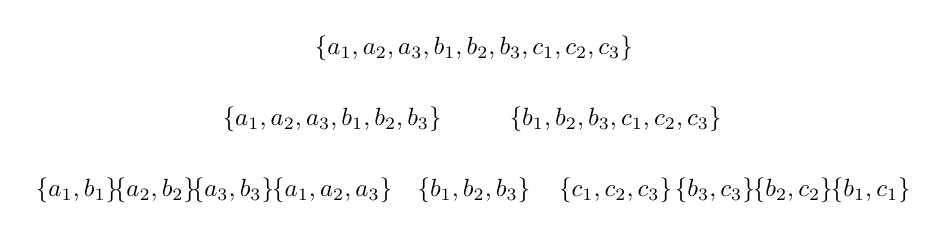
\begin{tikzpicture}[scale=.9, transform shape]
        \tikzstyle{v}=[draw, circle, minimum size=0.75cm, font=\footnotesize]
        % \tikzstyle{b}=[draw, font=\footnotesize]
        \tikzstyle{b}=[]
        \tikzstyle{e}=[]

        \node[b] (c0) at (0,0) {$\{a_1,a_2,a_3,b_1,b_2,b_3,c_1,c_2,c_3\}$};
        \node[b] (c1a) at (-2,-1) {$\{a_1,a_2,a_3,b_1,b_2,b_3\}$};
        \node[b] (c1b) at (2,-1) {$\{b_1,b_2,b_3,c_1,c_2,c_3\}$};
        \node[b] (c2a) at (-2,-2) {$\{a_1,a_2,a_3\}$};
        \node[b] (c2b) at (0,-2) {$\{b_1,b_2,b_3\}$};
        \node[b] (c2c) at (2,-2) {$\{c_1,c_2,c_3\}$};
        \node[b] (c2ab1) at (-5.6,-2) {$\{a_1,b_1\}$};
        \node[b] (c2ab2) at (-4.5,-2) {$\{a_2,b_2\}$};
        \node[b] (c2ab3) at (-3.4,-2) {$\{a_3,b_3\}$};
        \node[b] (c2bc1) at (5.6,-2) {$\{b_1,c_1\}$};
        \node[b] (c2bc2) at (4.5,-2) {$\{b_2,c_2\}$};
        \node[b] (c2bc3) at (3.4,-2) {$\{b_3,c_3\}$};

        \tedge{c0}{c1a}{solid}{}{};
        \tedge{c0}{c1b}{solid}{}{};

        \tedge{c1a}{c2ab1}{solid}{}{};
        \tedge{c1a}{c2ab2}{solid}{}{};
        \tedge{c1a}{c2ab3}{solid}{}{};
        \tedge{c1a}{c2a}{solid}{}{};
        \tedge{c1a}{c2b}{solid}{}{};

        \tedge{c1b}{c2bc1}{solid}{}{};
        \tedge{c1b}{c2bc2}{solid}{}{};
        \tedge{c1b}{c2bc3}{solid}{}{};
        \tedge{c1b}{c2b}{solid}{}{};
        \tedge{c1b}{c2c}{solid}{}{};
    \end{tikzpicture}

    \caption{}
\end{subfigure}

\caption{(a) Two doublets ($C2\times C3$), $\{a_1,a_2,a_3,b_1,b_2,b_3\}$ and $\{b_1,b_2,b_3,c_1,c_2,c_3\}$, intersecting on the triangle $\{b_1,b_2,b_3\}$. (b) The optimal DR-plan of the graph if we consider it to be a 2D graph; omits further decomposition of the three triangles into their edges and of edges into their individual nodes.}
\label{doublets}
\end{figure*}



\begin{example}
    In figure \ref{doublets}, the two well-constrained vertex-maximal proper subgraphs of the graph are the two doublets, shown in the second level of the DR-plan. These intersect on the well-constrained graph $\{b_1,b_2,b_3\}$. This will necessarily be a child $N=2$ levels below the parent of the two doublets, as explained in Theorem \ref{theorem:main_wellconstrained}. Also shown is the decomposition of the individual doublets. These have five well-constrained vertex-maximal proper subgraphs, the two triangles and the three edges connecting them. As explained in Theorem \ref{theorem:main_trivial}, all of them must be included in the optimal DR-plan. Were any left out, the union of the children would not be the entire parent.
\end{example}



\begin{figure*}\centering
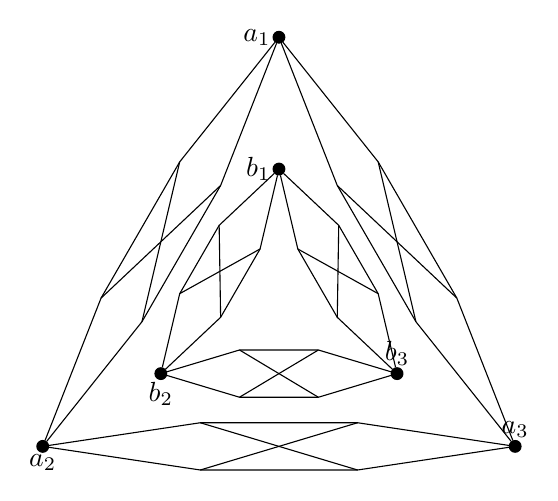
\begin{tikzpicture}[scale=3]
    \tikzstyle{v}=[draw, circle, minimum size=0.75cm]
    \tikzstyle{c}=[draw, circle, inner sep=1.5, fill=black]
    \tikzstyle{e}=[]

    \node[circle,fill=white,inner sep=7] (center) at (0,0-.125-.1) {};

    \node[c] (v1) at (0,0.866) [label={left,inner sep=.555}:$a_1$]{};
    \node[c] (v2) at (-1,-0.866) [label={below,inner sep=.555}:$a_2$]{};
    \node[c] (v3) at (1,-0.866) [label={above,inner sep=.555}:$a_3$]{};

    \node[c] (v4) at (0,0.433-.125) [label={left,inner sep=.555}:$b_1$]{};
    \node[c] (v5) at (-0.5,-0.433-.125) [label={below,inner sep=.555}:$b_2$]{};
    \node[c] (v6) at (0.5,-0.433-.125) [label={above,inner sep=.555}:$b_3$]{};

    \tedge{v1}{v2}{solid}{}{};
    \tedge{v1}{v3}{solid}{}{};
    \tedge{v2}{v3}{solid}{}{};

    \tedge{v4}{v5}{solid}{}{};
    \tedge{v4}{v6}{solid}{}{};
    \tedge{v5}{v6}{solid}{}{};


    \tedge{v1}{v4}{solid}{}{};
    \tedge{v2}{v5}{solid}{}{};
    \tedge{v3}{v6}{solid}{}{};


    \tedge{v4}{center}{dashed}{}{};
    \tedge{v5}{center}{dashed}{}{};
    \tedge{v6}{center}{dashed}{}{};


    % sin(30deg) = 0.5
    % cos(30deg) = 0.866

    % o/i -> outside/inside triangle
    % b/l/r -> bottom/left/right edge of triangle

    \coordinate (ob0) at (-0.333,-0.866-0.1);
    \coordinate (ob1) at (0.333,-0.866-0.1);
    \coordinate (ob2) at (-0.333,-0.866+0.1);
    \coordinate (ob3) at (0.333,-0.866+0.1);
    \draw (v2) -- (ob0) -- (ob1) -- (v3);
    \draw (v2) -- (ob2) -- (ob3) -- (v3);
    \draw (ob0) -- (ob3);
    \draw (ob2) -- (ob1);

    \draw[rotate around={60:(-1,-0.866)}] (v2) -- (-0.333,-0.766) -- (0.333,-0.766) -- (v1);
    \draw[rotate around={60:(-1,-0.866)}]  (v2) -- (-0.333,-0.966) -- (0.333,-0.966) -- (v1);
    \draw[rotate around={60:(-1,-0.866)}]  (-0.333,-0.766) -- (0.333,-0.966);
    \draw[rotate around={60:(-1,-0.866)}]  (-0.333,-0.966) -- (0.333,-0.766);

    \draw[rotate around={-60:(1,-0.866)}] (v3) -- (0.333,-0.766) -- (-0.333,-0.766) -- (v1);
    \draw[rotate around={-60:(1,-0.866)}]  (v3) -- (0.333,-0.966) -- (-0.333,-0.966) -- (v1);
    \draw[rotate around={-60:(1,-0.866)}]  (-0.333,-0.766) -- (0.333,-0.966);
    \draw[rotate around={-60:(1,-0.866)}]  (-0.333,-0.966) -- (0.333,-0.766);




    \coordinate (ib0) at (-0.167,-0.433-.125-0.1); %(-.167,-.658)
    \coordinate (ib1) at (0.167,-0.433-.125-0.1); %(.167,-.658)
    \coordinate (ib2) at (-0.167,-0.433-.125+0.1);%(-.167,-.458)
    \coordinate (ib3) at (0.167,-0.433-.125+0.1);%(.167,-.458)
    \draw (v5) -- (ib0) -- (ib1) -- (v6);
    \draw (v5) -- (ib2) -- (ib3) -- (v6);
    \draw (ib0) -- (ib3);
    \draw (ib2) -- (ib1);

    \draw[rotate around={60:(-0.5,-0.558)}] (v5) -- (-.167,-.658) -- (.167,-.658) -- (v4);
    \draw[rotate around={60:(-0.5,-0.558)}]  (v5) -- (-.167,-.458) -- (.167,-.458) -- (v4);
    \draw[rotate around={60:(-0.5,-0.558)}]  (-.167,-.658) -- (.167,-.458);
    \draw[rotate around={60:(-0.5,-0.558)}]  (-.167,-.458) -- (.167,-.658);

    \draw[rotate around={-60:(0.5,-0.558)}] (v6) -- (.167,-.658) -- (-.167,-.658) -- (v4);
    \draw[rotate around={-60:(0.5,-0.558)}]  (v6) -- (.167,-.458) -- (-.167,-.458) -- (v4);
    \draw[rotate around={-60:(0.5,-0.558)}]  (-.167,-.658) -- (.167,-.458);
    \draw[rotate around={-60:(0.5,-0.558)}]  (-.167,-.458) -- (.167,-.658);
% \newcommand{\tedge}[5]{\draw[#3] (#1)-- node[e, #5] (e#4) {#4} (#2)}

    % \draw (-1,-0.866) -- (-0.333,-0.966);

\end{tikzpicture}

\caption{A doublet with each edge replaced by a $K3,3$. \todo{Drawing incomplete.}}
\label{c2c3ofk33s}
\end{figure*}

\begin{example}
    In figure \ref{c2c3ofk33s}... \todo{Is it worth working through this? The first example has trivial and non-trivial.}
\end{example}





% \subsection{Extensions}
% This framework immediately pushes through for body-pin systems via a simple reduction. If there are $N$ pins on a body, it can be represented as a 2-tree with $N$ vertices, each corresponding to a pin, making sure to select edge distances such that the distance between pins is preserved. E.g.\ a body with two pins is an edge, three pins is a triangle, etc. Any bodies that share a pin now intersect on their vertex that corresponds to that pin. Now we have a bar-joint representation of the body-pin system in 2D and all proofs follow.

% With more effort, it can be shown that pinned line-incidence systems can also use this framework. This is done in section \ref{XXX}.



\subsection{Algorithm}
The algorithm to find the optimal DR-plan is a straightforward application of the theory. It begins by finding the well-constrained vertex-maximal proper subgraphs of the input well-constrained graph. If the intersection of any two of the subgraphs is well-constrained, then take those two to be children of the graph. Otherwise, all the subgraphs are the children. Apply recursively to the children. This naturally terminates when you reach trivial subgraphs.
